\documentclass[a4paper,10pt]{article}
\usepackage[utf8]{inputenc}
\usepackage{dsfont, graphicx,color}

%opening
\title{Incomplete quantum tomography using neural networks}
\author{Olivia Di Matteo}

\begin{document}

\maketitle

\section{Problem formalism}

The goal of quantum tomography is, given (many identical copies of) some arbitrary quantum state, take a series of measurements in order to determine its density matrix. When the dimension of the system $d$ is prime ($p$), or power of prime ($p^n$), a complete set of $d + 1$ bases that are mutually unbiased comprise an optimal set of measurements. These can be written in vector form, but another common way of expressing them is as $d + 1$ sets of $d - 1$ commuting observables (total of $d^2-1$) which have as mutual eigenvectors bases that are MU.

A density matrix $\rho$ can be expressed in terms of $d^2 - 1$ parameters; while an arbitrary complex $d \times d$ matrix contains $2d^2$ entries, the hermiticity and the condition on the trace of a density matrix, i.e. $\hbox{Tr}(\rho) = 1$ reduce the number of parameters required. A convenient way of expressing the density matrix is in terms of its expansion coefficients in an operator basis:
\begin{equation}
 \rho = \frac{1}{d} \mathds{1} + \frac{1}{d} \sum_{i = 1}^{d^2 - 1} a_i \Lambda_i 
\end{equation}
\noindent The operators in the basis should be traceless, and trace orthogonal $\hbox{Tr}(\Lambda_i \Lambda_j) = c \delta_{ij}$. Furthermore, if they are Hermitian, the  coefficients $a_i = \hbox{Tr}( \rho \Lambda_i )$ will be real. The canonical example is of course when $d = 2$ and $\Lambda = \{ \sigma_x, \sigma_y, \sigma_z \}$, so that the vector $\mathbf{a} = (a_1, a_2, a_3)$ is simply the 2-dimensional Bloch vector. 

The goal of a tomographic process would then be, given some measurement data, to determine the values of the coefficients $a_i$, and consequently $\rho$. \emph{In what follows, we focus exclusively on the special case where $\rho$ is a unknown random pure state.}

\section{Basic version: Incomplete tomography using neural networks}

If we consider multi-qubit systems, i.e. $d = 2^n$, the number of measurements required scales poorly with the number of qubits. As larger numbers of qubits become experimentally tractable, we will need effective methods of incomplete tomography to make the reconstruction process feasible. Efforts in this direction have involved compressed sensing, and least-bias maximum-likelihood state estimation (LBMLE). We propose here a method based on neural networks. The idea here is that the networks can be trained to reconstruct states based on simulated incomplete experimental data; this allows the heavy lifting to be done computationally, as one needs only train the network once, and then feed it the ``real'' experimental results. There is also a huge amount of versatility as one can simply adapt the process to train using whatever measurements are taken in a particular experimental setup.

We propose a basic feed-forward neural network for this task, shown in figure \ref{fig:nn}. The input layer consists of measurement frequencies for the measured bases. These are generated `experimentally' by computing the set of projectors for each basis, and the probability of that outcome via the Born rule. Then we use MC simulation to generate frequencies of each outcome (10000 points seems to give us frequencies pretty close to the original). The output layer consists of the basis coefficients above, the $a_i$.

\begin{figure}
 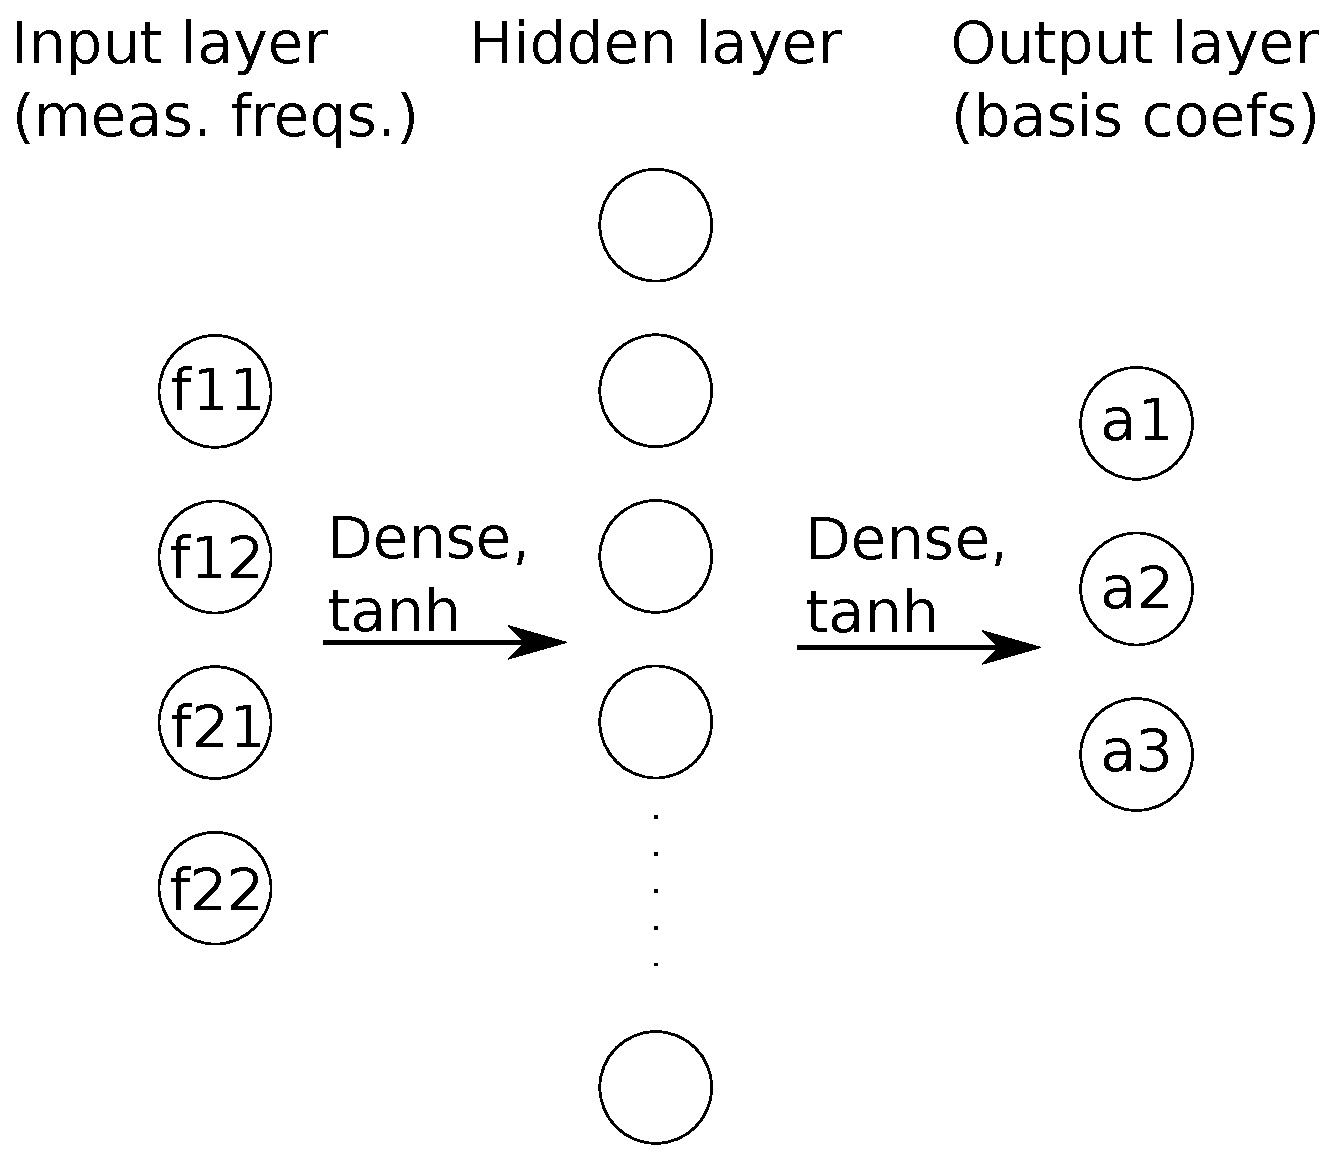
\includegraphics[scale=0.5]{nn_schematic}
 \caption{Simple diagram of neural network. The measurement frequencies from each measured basis are passed in as input nodes. The hidden layer seems to work well with a quadratic number of nodes, after which there are diminishing returns. The output layer should have $d^2 - 1$ nodes.}
 \label{fig:nn}
\end{figure}


Through experimentation we need to determine the properties of the hidden layer(s) that are the most effective for this purpose. So far things that work well are:
\begin{itemize}
\item {We choose tanh as the activation function, as it takes a range (-1, 1) and the $a_i$ can be positive or negative.}
\item {We choose the cosine proximity as the loss function; this is physically motivated, as in the single-qubit case it can be thought of as the angle between Bloch vectors, which one should try to minimize to get as close as possible to the true state.}
\item {We use a single hidden layer. Adding more seems to give us no benefits, except for longer coffee breaks while the code runs.}
\item {The networks are trained using data taken from Haar-random pure states.}
\end{itemize}

\noindent We also need a way to quantify the performance of the network. We choose the \textbf{fidelity}, however there are a few hiccups here:
\begin{itemize}
 \item{The output of the network is not always normalized. As we assume we are working strictly with pure states, before computing the fidelity we normalize the vectors.}
 \item{Once normalized, the state is not necessarily a valid quantum state, i.e. is not positive semidefinite (PSD), in particular for $d > 2$. In cases I have looked at, there is some very tiny non-zero eigenvalue, even in the single qubit case. Therefore to get a physical state estimation we should look to the closest PSD matrix.}
\end{itemize}


\section{1 qubit}

As proof of concept, we train the network to reconstruct a single qubit pure state. We use a single hidden layer of size 64 (input size is 6 for all bases, 4 for two bases, and output size is always 3). We trained our network with 9000 Haar-random pure states, and tested on 1000 additional ones.

Training the network with all 3 MUBs yields an average fidelity of 0.9999, which is a solid sanity check. We then attempt to train it using simulated measurement data from only 2 of the 3 MUBs. The network takes only a second or two to train (data generation and comparison with LBMLE takes far longer!). Our network reconstructs states with a fidelity of 0.944 on average; this can be compared, using the same test data, with the LBMLE algorithm, which reconstructs the states with an average of 0.91. Results are discussed in more detail in Section \ref{sec:angdep}.

\textcolor{red}{To do: plots of dependence of fidelity on hidden layer size, and on number of training data points}

\section{1 qutrit}

We choose as our operator basis the Gell-Mann matrices. The qutrit is an interesting case because density matrices constructed using arbitrary vectors of norm 1 are Hermitian and have trace 1, but are not necessarily PSD. As a consequence there has been a lot of work done in attempt to characterize the regions of the qutrit Bloch sphere that produce `legal' states (add references).

Regardless of this fact, it seems that the neural network is able to learn quite well how to reconstruct qutrit states. We train again using largely the same parameters as the qubit case: 10000 Haar-random pure states split 9000/1000, and still a hidden layer of size 64. States that are not PSD after reconstruction are kicked over to the closest PSD state.

I put the results in Table \ref{tab:qutrit}. Measuring all 4 bases of course reconstructs the states with fidelity close to 1, so I've not included this in the table. With 3 bases, the two algorithms perform comparably with an average fidelity of around 0.958. What is more interesting is that when we measure in only 2 bases, the network begins to perform better.

\begin{table}[h!]
 \centering
 \begin{tabular}{|c||c|c|c|}
 \hline
  Num. meas. bases &  Fidelity NN & Fidelity LBMLE \\ \hline
  3 & 0.9582 &  0.9580 \\
  2 & 0.8978 & 0.8547  \\ \hline
 \end{tabular}
 \caption{Fidelity using incomplete measurements. Here I averaged together results of all choices of 2/3 bases, as they weren't really too different.}
 \label{tab:qutrit}
\end{table}

\section{2 qubits}

This is where I'm stuck. So far nothing I've tried seems to work. Average reconstruction fidelity with all 5 MUBs seems stuck at around 0.83. Things that do not work are:
\begin{itemize}
 \item Adding more hidden layers
 \item Changing the size of the hidden layer(s)
 \item Changing the operator basis; I've tried the Pauli basis (which has tensor product structure) and also the generalized Gell-Mann matrices (which do not)
\end{itemize}

I have a few lines of investigation to follow here and will try more stuff out.

\section{Next questions}
 Some obvious questions to consider next:
 \begin{itemize} 
  \item Why aren't things working in dimension 4? Is there a problem with composite systems?
  \item What happens for mixed states? Does the neural network still fare well? We cannot normalize it now, it may live inside the Bloch sphere. How do we ensure that the output is always a vector with norm $< 1$ still close to the original state?
 \end{itemize}
 
 
\section{Angular dependence of single qubit reconstructions} \label{sec:angdep}

\textcolor{red}{This is some interesting stuff that goes beyond the scope of doing tomo with neural networks, and focuses more on the specific choice of measurements in an incomplete tomography setting. However it's still quite a neat result, and allows us to see where exactly the neural network is outperforming the existing algorithm.}

One important thing to consider is the quality of the data set that goes into the network training. We used Haar-random states (HRS), which are generated by hitting a fiducial state by a Haar-random unitary (HRU). HRUs are distributed in a distinct way; in particular, the ``weight" factor in the measure of integration is 
\begin{equation} 
 dU \simeq \sin \beta d\alpha d\beta d\gamma
\end{equation}
where $\alpha, \beta, \gamma$ are the 3 parameters which allow us to construct the matrix
\begin{equation}
 U(\alpha, \beta, \gamma) = \left( 
  \begin{array}{cc}
   e^{i \alpha} \cos( \beta/2) & -e^{i \gamma} \sin(\beta / 2) \\
    e^{-i \gamma} \sin(\beta / 2) & e^{-i \alpha} \cos( \beta/2) 
  \end{array}
  \right)
\end{equation}
 (more technically this is SU(2) rather than U(2) I guess). This looks very similar to the integration measure in spherical coordinates, when integrating over a sphere of radius 1. In this sense, $\beta$ plays the role of the polar angle $\theta$. The extra factor of $\sin \beta$ takes its maximum value at $\beta = \pi / 2$, namely at the equator of the sphere; there is consequently more `weight' added to these states, meaning that \emph{equatorial states are more likely to occur than, say, polar states, when randomly sampling from the distribution of HRUs}.
 
 To that end, I was initially concerned that using a training dataset based on HRS would mean that there are more states around the equator, and that consequently we would be able to learn these states better than the polar states. So I decided to plot the polar angle of the states on the Bloch sphere vs the fidelity of the reconstruction from the two different methods. I did this for all 3 combinations of measurement bases, ZY, XY, and ZX. Results for ZY and ZX were practically identical; the main differences lie between e.g. ZY and XY.
 
 The first thing to note is that it doesn't seem that the distribution of the data set has much effect; I make this conclusion because when we reconstruct with the ZY bases, the states in the middle (i.e. angle ~ $\pi/2$) are more poorly reconstructed than the polar states, despite there being more of them in the training set (see, for example, the distribution of fidelities of \ref{fig:fid_v_angle_zy}. What \emph{does} make a huge difference is the bases we choose to measure in.
 
 The X and Y axes are those defining the equator of the Bloch sphere, and so it makes sense that measuring in those bases will give us better reconstructions simply because there is more `room to move around' in this portion of the sphere. There is, in a sense, greater chance for error here and so we want to learn as much as we can about how things related to these two axes vs. the polar one. 
 
 What's more interesting though is the differences between the two algorithms. The average fidelity for the neural network is pretty much the same whether we use ZY or XY. However for both algorithms, the fidelity for the XY case is far more correlated with angle. The LBMLE looks normally distributed in both cases but for the ZY measurements the normal distribution is filled in, while for XY the points simply follow the outline of a bell curve. 
 
 For the ZY case, the neural network looks like it fares worse closer to the middle (which I feel makes sense as we are using the cosine proximity as a loss function). However the average is still superior because the fidelity of the polar states is handled better than in LBMLE. In the XY case again the NN handles the polar states better, and it looks more paraboloid than it does normal. \\
 
 
 \begin{figure}[h]
  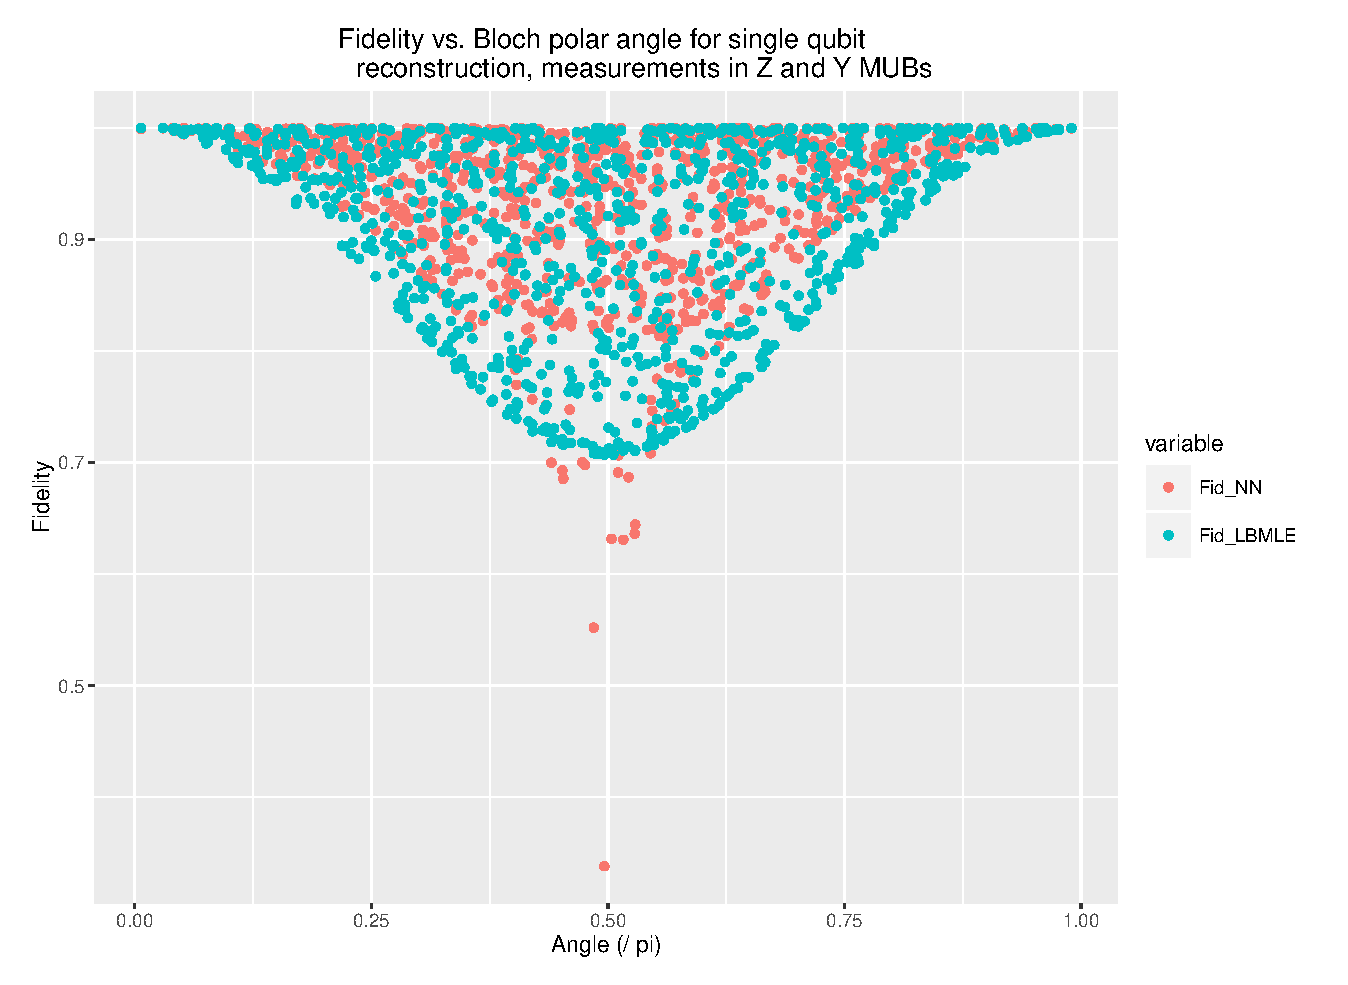
\includegraphics[scale=0.6]{fid_v_angle_zy}
  \caption{Fidelity of reconstruction vs angle with measurement data from the Z and Y MUBs. The red points are those of the neural network, and blue for the least-bias estimation.}
  \label{fig:fid_v_angle_zy}
 \end{figure}
 
  \begin{figure}[h]
  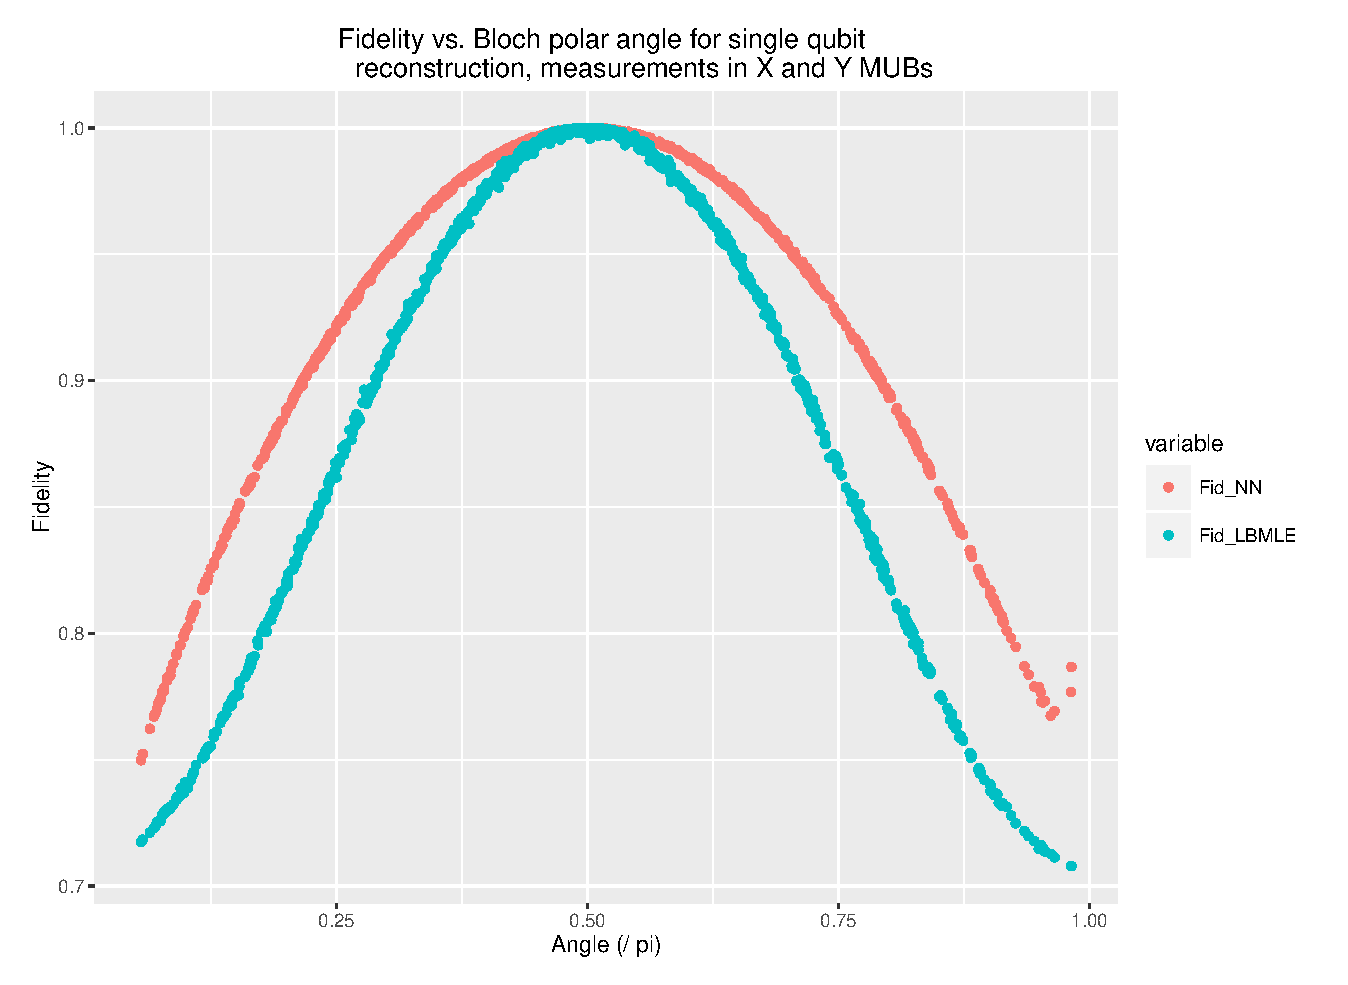
\includegraphics[scale=0.6]{fid_v_angle_xy}
  \caption{Fidelity of reconstruction vs angle with measurement data from the X and Y MUBs. Seems to be highly correlated with angle. The neural networks average fidelity seems to get a boost from its ability to better reconstruct the states closer to the poles of the Bloch sphere.}
  \label{fig:fid_v_angle_xy}
 \end{figure}
 
\end{document}
